\documentclass[xetex,mathserif,serif,handout]{beamer}

\usepackage{xunicode}
\usepackage{xltxtra}
\usepackage{color}
\usepackage{url}
\usepackage{listings}
\usepackage{fontspec}
\usepackage{geometry}
\usepackage{lastpage}
\usepackage{fancyhdr}
\usepackage{amsmath}
\usepackage{amsthm}
\usepackage{amssymb}
\usepackage{blkarray}
\usepackage{multicol}
\usepackage{relsize}

\definecolor{solarized@base03}{HTML}{002B36}
\definecolor{solarized@base02}{HTML}{073642}
\definecolor{solarized@base01}{HTML}{586e75}
\definecolor{solarized@base00}{HTML}{657b83}
\definecolor{solarized@base0}{HTML}{839496}
\definecolor{solarized@base1}{HTML}{93a1a1}
\definecolor{solarized@base2}{HTML}{EEE8D5}
\definecolor{solarized@base3}{HTML}{FDF6E3}
\definecolor{solarized@yellow}{HTML}{B58900}
\definecolor{solarized@orange}{HTML}{CB4B16}
\definecolor{solarized@red}{HTML}{DC322F}
\definecolor{solarized@magenta}{HTML}{D33682}
\definecolor{solarized@violet}{HTML}{6C71C4}
\definecolor{solarized@blue}{HTML}{268BD2}
\definecolor{solarized@cyan}{HTML}{2AA198}
\definecolor{solarized@green}{HTML}{859900}
\definecolor{yaleblue}{HTML}{0E4C92}

\setbeamertemplate{navigation symbols}{}
% \setbeamerfont{title}{family=\old}
% \setbeamerfont{author}{family=\tfont}%
% \setbeamerfont{frametitle}{family=\oldA}
% \setbeamerfont{date}{family=\dfont}

\setbeamertemplate{itemize items}{--}
\setbeamercolor*{item}{fg=black}

\defaultfontfeatures{Mapping=tex-text}
\hypersetup{pdfstartview={FitH}}

\newcommand{\old}[1]{\fontspec[Alternate=1,Ligatures={Common}]{Hoefler Text}\fontsize{18pt}{30pt}\selectfont #1}%
\newcommand{\oldA}[1]{\fontspec[Alternate=1,Ligatures={Common, Rare}]{Hoefler Text}\fontsize{12pt}{15pt}\selectfont #1}%
\newcommand{\oldB}[1]{\fontspec[Ligatures={Common}]{Didot}\fontsize{12pt}{15pt}\color{solarized@base02}\selectfont #1}%
\newcommand{\tfont}[1]{\fontspec[Alternate=1,Ligatures={Common}]{Hoefler Text}\fontsize{12pt}{20pt}\selectfont #1}%
\newcommand{\dfont}[1]{\fontspec[Ligatures={Common}]{Didot}\fontsize{12pt}{12pt}\selectfont #1}%

\newcommand{\minimize}{\mathop{\mathrm{minimize}}}
\newcommand{\argmin}{\mathop{\mathrm{arg\,min}}}
\newcommand{\argmax}{\mathop{\mathrm{arg\,max}}}
\newcommand{\st}{\mathop{\mathrm{subject\,\,to}}}

\newcommand\independent{\protect\mathpalette{\protect\independenT}{\perp}}
\def\independenT#1#2{\mathrel{\rlap{$#1#2$}\mkern2mu{#1#2}}}

\setlength{\parindent}{0pt}
\setlength{\parskip}{12pt}

\setromanfont [Ligatures={Common}, Numbers={OldStyle}, Variant=01,
 BoldFont={LinLibertine_RB.otf},
 ItalicFont={LinLibertine_RI.otf},
 BoldItalicFont={LinLibertine_RBI.otf}
 ]{LinLibertine_R.otf}



\begin{document}

%%%%%%%%%%%%%%%%%%%%%%%%%%%%%%%%%%%%%%%%%%%%%%%%%%%
\begin{frame}[fragile] \frametitle{}

\vfill

{\fontsize{0.7cm}{0cm}\selectfont Lecture 17 \\\vspace{0.2cm}
Intro to Lasso Regression}\\\vspace{0.5cm}
11 November 2015

\vspace{2cm}

\begin{minipage}{0.6\textwidth}
Taylor B. Arnold \\
Yale Statistics \\
STAT 312/612
\end{minipage}
\hfill
\begin{minipage}{0.3\textwidth}\raggedleft

\includegraphics[scale=0.3]{../yale-logo.png}
\end{minipage}%

\end{frame}

%%%%%%%%%%%%%%%%%%%%%%%%%%%%%%%%%%%%%%%%%%%%%%%%%%%
\begin{frame}[fragile] \frametitle{}

{\color{yaleblue}\fontsize{16pt}{20pt}\selectfont Notes}

\begin{itemize}
\item problem set 5 posted; due today
\end{itemize}

\end{frame}

%%%%%%%%%%%%%%%%%%%%%%%%%%%%%%%%%%%%%%%%%%%%%%%%%%%
\begin{frame}[fragile] \frametitle{}

{\color{yaleblue}\fontsize{16pt}{20pt}\selectfont Goals for today}

\begin{itemize}
\item introduction to lasso regression
\item the subdifferential
\item basics of the lars algorithm
\end{itemize}

\end{frame}

%%%%%%%%%%%%%%%%%%%%%%%%%%%%%%%%%%%%%%%%%%%%%%%%%%%
\begin{frame}[fragile] \frametitle{}

{\color{yaleblue}\fontsize{16pt}{20pt}\selectfont Lasso Regression }

\end{frame}

%%%%%%%%%%%%%%%%%%%%%%%%%%%%%%%%%%%%%%%%%%%%%%%%%%%
\begin{frame}[fragile] \frametitle{}

Two lectures ago, I introduced the ridge estimator:
\begin{align*}
\widehat{\beta}_\lambda &= \argmin_b \left\{ || y - Xb ||_2^2 + \lambda ||b||_2^2 \right\}
\end{align*}
\pause Notice that for any $\lambda > 0$ there exists an $s_\lambda$ equal
to $||\widehat{\beta}_\lambda||_2^2$ where:
\begin{align*}
\widehat{\beta}_\lambda &= \argmin_b \left\{ || y - Xb ||_2^2, \quad \text{s.t.} \quad || b ||_2^2 \leq s_\lambda \right\}
\end{align*}
\pause This is the dual form of the optimization problem (essentially, the
opposite of using Lagrangian multipliers).

\end{frame}

%%%%%%%%%%%%%%%%%%%%%%%%%%%%%%%%%%%%%%%%%%%%%%%%%%%
\begin{frame}[fragile] \frametitle{}

Lasso regression replaces the $\ell_2$ penalty with an $\ell_1$ penalty,
and looks deceptively similar to the ridge regression:
\begin{align*}
\widehat{\beta}_\lambda &= \argmin_b \left\{ || y - Xb ||_2^2 + \lambda ||b||_1 \right\}
\end{align*}
Where the $\ell_1$-norm is defined as the sum of the absolute values of the
vector's components:
\begin{align*}
|| \beta ||_1 &= \sum_i | \beta_i |
\end{align*}
\pause Similarly, for any $\lambda > 0$ there exists an $s_\lambda$ equal
to $||\widehat{\beta}_\lambda||_1$ where:
\begin{align*}
\widehat{\beta}_\lambda &= \argmin_b \left\{ || y - Xb ||_2^2, \quad \text{s.t.} \quad || b ||_1 \leq s_\lambda \right\}
\end{align*}

\end{frame}

%%%%%%%%%%%%%%%%%%%%%%%%%%%%%%%%%%%%%%%%%%%%%%%%%%%
\begin{frame}[fragile] \frametitle{}

The change in the norm of the penalty may seem like only a
minor difference, however the behavior of the $\ell_1$-norm
is significantly different than that of the $\ell_2$-norm.

\pause A classic illustration, with $p=2$ and using the dual
form of the estimators, shows exactly how this comes about.

\end{frame}

%%%%%%%%%%%%%%%%%%%%%%%%%%%%%%%%%%%%%%%%%%%%%%%%%%%
\begin{frame}[fragile] \frametitle{}

\begin{center}
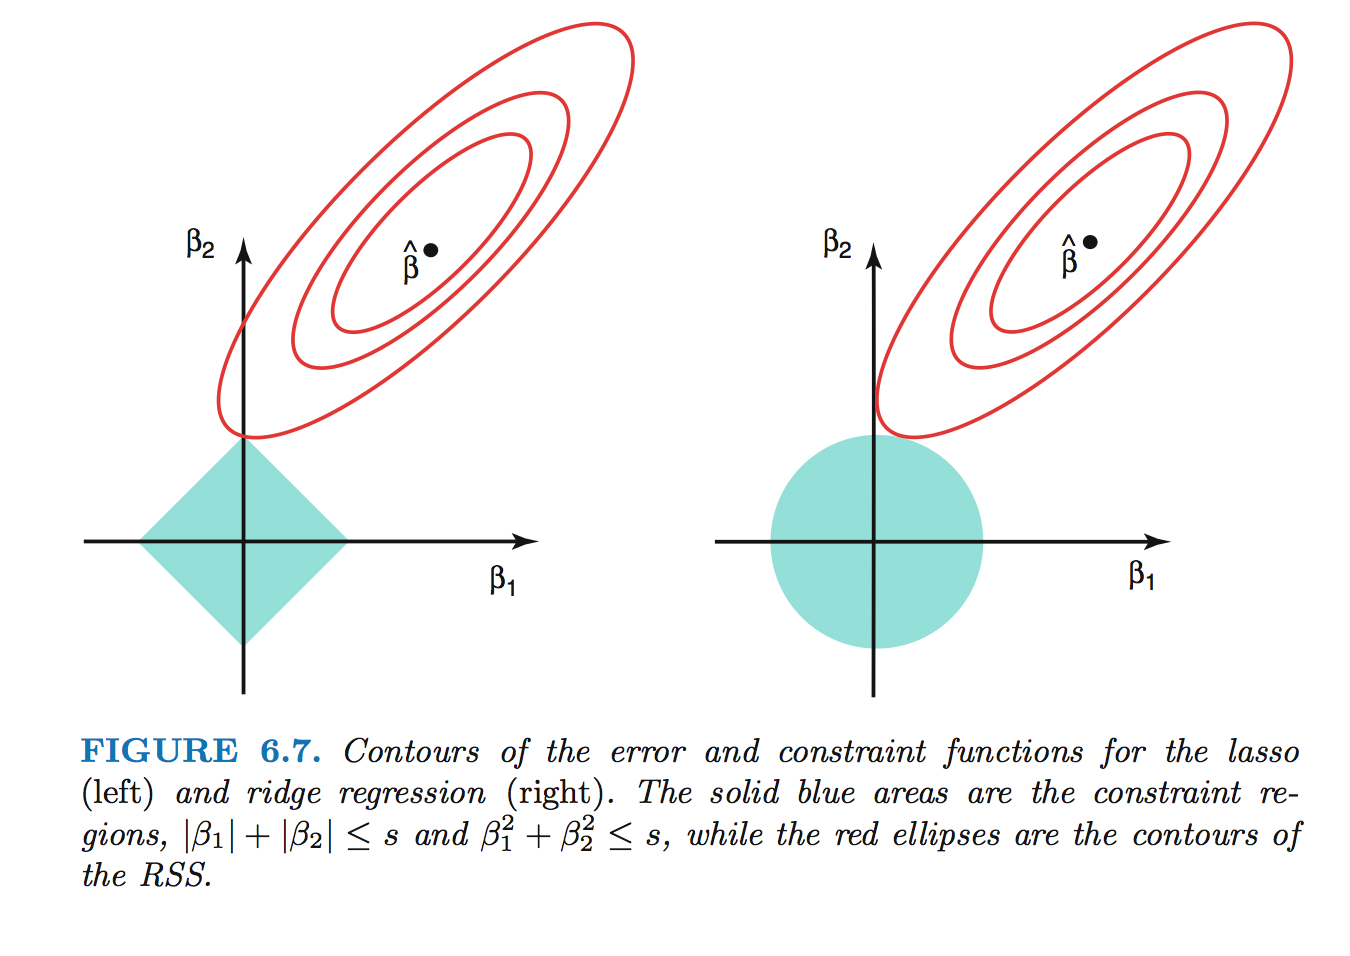
\includegraphics[width=\textwidth]{img/img01.png}
\end{center}

\end{frame}

%%%%%%%%%%%%%%%%%%%%%%%%%%%%%%%%%%%%%%%%%%%%%%%%%%%
\begin{frame}[fragile] \frametitle{}

I think of there being three major difference between ridge
and lasso:
\begin{enumerate}
\item the sharp, non-differentiable corners of the $\ell_1$-ball
produce parsimonious models for sufficiently large values of $\lambda$ \pause
\item the lack of rotational invariance limits the use of the singular
value theory that is so useful in unpenalized and ridge regression \pause
\item the lasso lacks an analytic solution, making both computation
and theoretical results more difficult
\end{enumerate}

\end{frame}

%%%%%%%%%%%%%%%%%%%%%%%%%%%%%%%%%%%%%%%%%%%%%%%%%%%
\begin{frame}[fragile] \frametitle{}

At the start of this semester, most of you had already worked with
multivariate regression, and many had even seen ridge, PCR, and lasso
regression.

\pause By looking at these techniques at a deeper level with the
help of matrix analysis you have (hopefully) seen that there is a
substantial amount of nuance that is not immediately obvious.

\pause The lasso is very much the same (in that there is significant depth beyond what
you would see in a first pass), but the lack of differentiability and
rotational invariance make most matrix methods insufficient. Instead
we will be looking to \textit{convex analysis} for tools of study to
use in the remainder of the semester.

\end{frame}

%%%%%%%%%%%%%%%%%%%%%%%%%%%%%%%%%%%%%%%%%%%%%%%%%%%
\begin{frame}[fragile] \frametitle{}

In slight reverse of the other techniques, we are going to study
the lasso in the following order:
\begin{enumerate}
\item computation
\item application
\item theory
\end{enumerate}
With additional computational considerations to follow, time
permitting.

\end{frame}

%%%%%%%%%%%%%%%%%%%%%%%%%%%%%%%%%%%%%%%%%%%%%%%%%%%
\begin{frame}[fragile] \frametitle{}

Ordinary least squares and ridge regression have what are called
\textit{analytic solutions}, we can write down an explicit formula
for what the estimators are.

\pause Generalized linear models, on the other hand, have only
\textit{numerical solutions} with iterative methods. We have algorithm
that, when run sufficiently long enough should yield a solution with
a reasonable accuracy.

\pause The lasso falls somewhere in-between these two cases, as it
has a \textit{direct numerical solution}. We cannot write out an
explicit analytic form, but the algorithm is not iterative and would
yield the exact solution given a machine with infinite precision.

\end{frame}

%%%%%%%%%%%%%%%%%%%%%%%%%%%%%%%%%%%%%%%%%%%%%%%%%%%
\begin{frame}[fragile] \frametitle{}

{\color{yaleblue}\fontsize{16pt}{20pt}\selectfont The subdifferential}

\end{frame}

%%%%%%%%%%%%%%%%%%%%%%%%%%%%%%%%%%%%%%%%%%%%%%%%%%%
\begin{frame}[fragile] \frametitle{}

The lasso solution does not have a derivative for any point where $\beta_j$ is
equal to zero. We instead use the concept of a \textit{subdifferential}.

\pause Let $h$ be a convex function. The subdifferential at point $x_0$ in the
domain of $h$ is equal to the set:
\begin{align*}
\partial(h)(x_0 ) &= \left\{ c \in \mathbb{R} \quad \text{s.t.} \quad c \leq \frac{h(x) - h(x_0)}{x - x_0} \quad \forall \quad x \in
\text{Dom}(h) \right\}
\end{align*}
Less formally, it is the set of all slopes which are tangent to the function at the point $x_0$.

\end{frame}


%%%%%%%%%%%%%%%%%%%%%%%%%%%%%%%%%%%%%%%%%%%%%%%%%%%
\begin{frame}[fragile] \frametitle{}

For example, the subdifferential of the absolute value function is
\begin{align*}
\partial(| \cdot |)(x) &= \left\{ \begin{array}{ll} -1, &x < 0 \\[0pt] [-1,1], &x = 0 \\ 1, &x > 0 \end{array} \right.
\end{align*}

\end{frame}

%%%%%%%%%%%%%%%%%%%%%%%%%%%%%%%%%%%%%%%%%%%%%%%%%%%
\begin{frame}[fragile] \frametitle{}

An illustration of elements of the subdifferential for a more complex
convex function:
\begin{center}
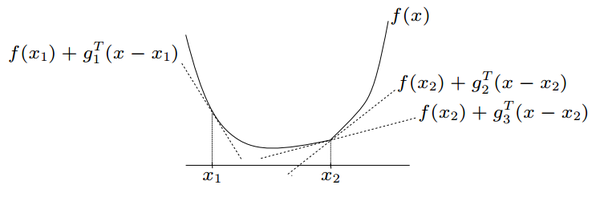
\includegraphics[width=\textwidth]{img/img02.png}
\end{center}

\end{frame}

%%%%%%%%%%%%%%%%%%%%%%%%%%%%%%%%%%%%%%%%%%%%%%%%%%%
\begin{frame}[fragile] \frametitle{}

As shown in the figure, the subdifferential can be generalized to
higher dimensions as follows:
\begin{align*}
\partial(h)(x_0) &= \left\{ g \in \mathbb{R}^p \quad \text{s.t.} \quad h(x_0) \geq h(x) + g^t (x - x_0) \quad \forall \quad x \in
\text{Dom}(h) \right\}
\end{align*}

\end{frame}

%%%%%%%%%%%%%%%%%%%%%%%%%%%%%%%%%%%%%%%%%%%%%%%%%%%
\begin{frame}[fragile] \frametitle{}

We will use three properties of the subdifferential of a convex
function $h$:
\begin{enumerate}
\item the gradient $\nabla(h)$ exists at the point $x_0$ if and only if
$\partial(h)(x_0)$ is equal to a single value, which is equal to $\nabla(h)(x_0)$ \pause
\item for every point $x_0$, the set $\nabla(h)(x_0)$ is a nonempty closed interval $[a,b]$ \pause
\item the point $x_0$ is a global minimum of $h$ if and only if the subdifferential
contains zero; in other words, $0 \in \partial(h)(x_0)$
\end{enumerate}

\end{frame}

%%%%%%%%%%%%%%%%%%%%%%%%%%%%%%%%%%%%%%%%%%%%%%%%%%%
\begin{frame}[fragile] \frametitle{}

{\color{yaleblue}\fontsize{16pt}{20pt}\selectfont Least angle regression}

\end{frame}

%%%%%%%%%%%%%%%%%%%%%%%%%%%%%%%%%%%%%%%%%%%%%%%%%%%
\begin{frame}[fragile] \frametitle{}

The algorithm for solving the exact form of the lasso comes from
\begin{quote}
Efron, Bradley, Trevor Hastie, Iain Johnstone, and Robert Tibshirani.
``Least angle regression." The Annals of Statistics 32, no. 2 (2004): 407-499.
\end{quote}
\pause Today, I will sketch out how the algorithm works in the simple case where
$X^tX$ is the identity matrix. Problem set $6$ illustrates how this works in the
more general case.

\end{frame}

%%%%%%%%%%%%%%%%%%%%%%%%%%%%%%%%%%%%%%%%%%%%%%%%%%%
\begin{frame}[fragile] \frametitle{}

The lasso equation is a convex function, so let us try to calculate the subdifferential
and determine what solution $\beta$ give us $\partial(h)(\beta)$ that contain $0$.

To simplify matters, assume that $X^tX$ is equal to the identity matrix. We will also
add a factor of $2$ to the penalty, so that it because $2 \lambda ||\beta||_1$.

\end{frame}

%%%%%%%%%%%%%%%%%%%%%%%%%%%%%%%%%%%%%%%%%%%%%%%%%%%
\begin{frame}[fragile] \frametitle{}

The lasso equation, in our simpler case, is given by:
\begin{align*}
f(b) &= || y - Xb ||_2^2 + 2 \lambda ||b||_1 \\
&= y^t y + b^t b - 2 y^t X b + 2 \lambda || b ||_1
\end{align*}
\pause We know that the gradient of the front terms is just $2b - 2 X^t y$,
and the subdifferential of the $\ell_1$ norm is equal to $\lambda$ times
that of the absolute value function.

\end{frame}

%%%%%%%%%%%%%%%%%%%%%%%%%%%%%%%%%%%%%%%%%%%%%%%%%%%
\begin{frame}[fragile] \frametitle{}

The $j$-th component of the subdifferential is then given by:
\begin{align*}
\partial(h)(b_j) &= \left\{ \begin{array}{ll}
2 b_j - 2 x_j^t y + 2 \lambda, &b_j > 0 \\[0pt]
[-2\lambda,2\lambda] - 2 x_j^t y, &b_j = 0 \\[0pt]
2 b_j - 2 x_j^t y - 2\lambda, &b_j < 0
\end{array} \right.
\end{align*}
So what would make these equal to zero for all $j$?

\end{frame}

%%%%%%%%%%%%%%%%%%%%%%%%%%%%%%%%%%%%%%%%%%%%%%%%%%%
\begin{frame}[fragile] \frametitle{}

If $b_j$ is greater than zero, we need the following to hold:
\begin{align*}
2 b_j - 2 x_j^t y + 2 \lambda &= 0 \\
b_j &= x_j^t y - \lambda
\end{align*}
\pause So $b_j$ is a linear function of $\lambda$, with an intercept of
$x_j^t y$ and a slope of $-\lambda$. \pause However this only holds when:
\begin{align*}
x_j^t y - \lambda &> 0 \\
x_j^t y &> \lambda
\end{align*}
So, for all $\lambda$ between $x_j^t y$ and $0$. So clearly $b_j$
can only be positive if $x_j^t y$ is positive.

\end{frame}

%%%%%%%%%%%%%%%%%%%%%%%%%%%%%%%%%%%%%%%%%%%%%%%%%%%
\begin{frame}[fragile] \frametitle{}

What if $b_j$ is less than zero? We instead need the following:
\begin{align*}
2 b_j - 2 x_j^t y - 2 \lambda &= 0 \\
b_j &= x_j^t y + \lambda
\end{align*}
Whenever:
\begin{align*}
x_j^t y + \lambda &< 0 \\
x_j^t y &< -\lambda\\
-x_j^t y &> \lambda
\end{align*}
As $\lambda > 0$, therefore, $b_j$ is only negative if
$x_j^t y$ is negative.

\end{frame}

%%%%%%%%%%%%%%%%%%%%%%%%%%%%%%%%%%%%%%%%%%%%%%%%%%%
\begin{frame}[fragile] \frametitle{}

We can combine these two conditions together, by
saying that whenever $\lambda < |x_j^t y|$ we have:
\begin{align*}
b_j &= x_j^t y - \text{sign}(x_j^t y) \cdot \lambda
\end{align*}

\end{frame}

%%%%%%%%%%%%%%%%%%%%%%%%%%%%%%%%%%%%%%%%%%%%%%%%%%%
\begin{frame}[fragile] \frametitle{}

What about the third case in the subdifferential?
If $b_j$ is equal to zero, we need:
\begin{align*}
0 &\in [-2\lambda,2\lambda] - 2 x_j^t y
\end{align*}
Which implies that both
\begin{align*}
-2\lambda - 2 x_j^t y &< 0 \\
\lambda &> - x_j^t y
\end{align*}
\pause and
\begin{align*}
2 \lambda - 2 x_j^t y &> 0 \\
\lambda &> x_j^t y
\end{align*}
hold.

\pause This can again be simplified into one equation,
which here yields $\lambda > |x_j^t y|$ whenever $b_j$ is
equal to zero.

\end{frame}

%%%%%%%%%%%%%%%%%%%%%%%%%%%%%%%%%%%%%%%%%%%%%%%%%%%
\begin{frame}[fragile] \frametitle{}

Now, amazingly, we have a full solution to the lasso equation
in the case where $X^t X$ is the identity matrix:
\begin{align*}
\widehat{\beta}^\lambda_j &= \left\{ \begin{array}{ll}
0, &\lambda > |x_j^t y| \\[0pt]
x_j^t y - \text{sign}(x_j^t y) \cdot \lambda, &\lambda \leq |x_j^t y| \\
\end{array} \right.
\end{align*}

\end{frame}

%%%%%%%%%%%%%%%%%%%%%%%%%%%%%%%%%%%%%%%%%%%%%%%%%%%
\begin{frame}[fragile] \frametitle{}

Let's construct a test dataset, with $X^tX$ equal
to the identity matrix. One easy way is with the
\texttt{poly} function, which produces an orthogonal
polynomial basis of an arbitrarily high order.
\begin{verbatim}
> n <- 1000
> p <- 5
> X <- poly(seq(0,1,length.out=n),degree=p)
> round(t(X) %*% X,6)
  1 2 3 4 5
1 1 0 0 0 0
2 0 1 0 0 0
3 0 0 1 0 0
4 0 0 0 1 0
5 0 0 0 0 1
> beta <- c(1,0,1,0,0)
> y <- X %*% beta + rnorm(n,sd=0.3)
\end{verbatim}
Notice that the regression vector has only $2$ non-zero components.

\end{frame}

%%%%%%%%%%%%%%%%%%%%%%%%%%%%%%%%%%%%%%%%%%%%%%%%%%%
\begin{frame}[fragile] \frametitle{}

Now we start by constructing a sequence of $\lambda$ values
to which we want to fit the model. We know the non-zero solutions
lie between $0$ and $||X^t y||_\infty$, so we'll pick twice that
range:
\begin{verbatim}
> Xty <- t(X) %*% y
> lambda <- seq(0,max(abs(Xty))*2,length.out=1e5)
\end{verbatim}

\end{frame}

%%%%%%%%%%%%%%%%%%%%%%%%%%%%%%%%%%%%%%%%%%%%%%%%%%%
\begin{frame}[fragile] \frametitle{}

The first element of $\widehat{\beta}$ can then be
simply calculated according to our formula.
\begin{verbatim}
> j <- 1
> beta <- Xty[j] - lambda * sign(Xty[j])
> beta[lambda > abs(Xty[j])] <- 0
\end{verbatim}
We then plot this as a \textit{path} of solutions with
respect to $\lambda$:
\begin{verbatim}
> plot(lambda, beta, type='l')
\end{verbatim}

\end{frame}

%%%%%%%%%%%%%%%%%%%%%%%%%%%%%%%%%%%%%%%%%%%%%%%%%%%
\begin{frame}[fragile] \frametitle{}

\begin{center}
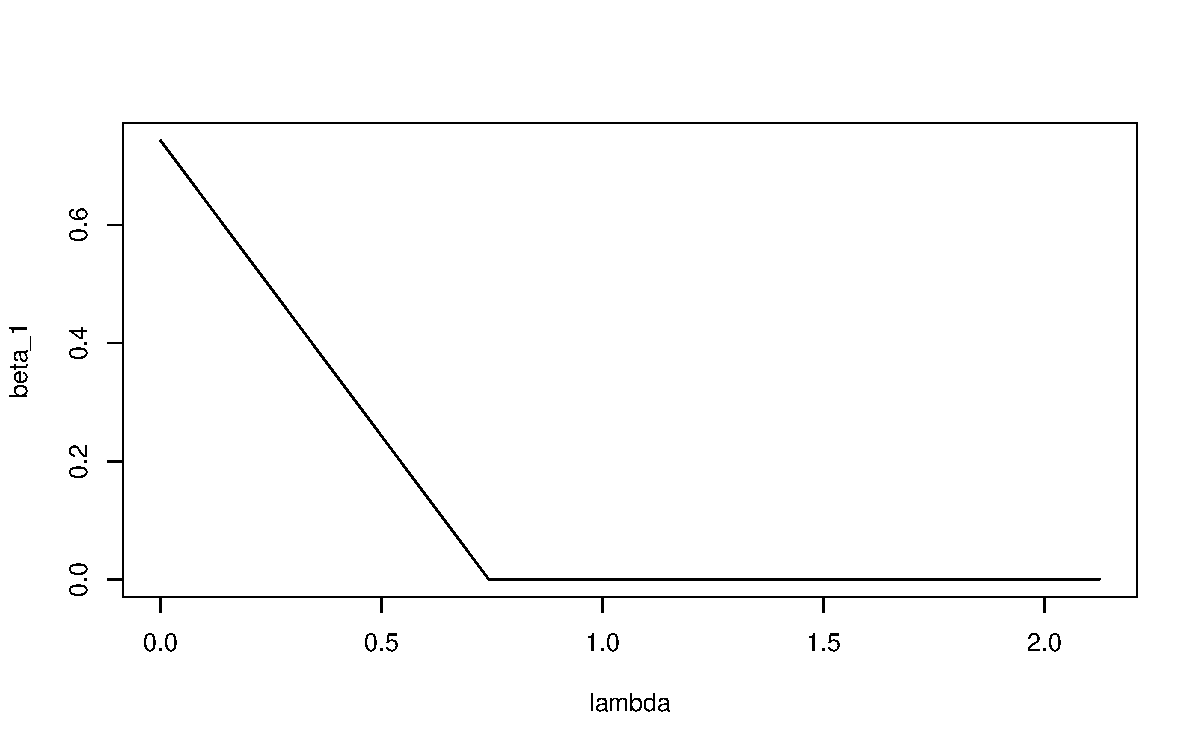
\includegraphics[width=\textwidth]{img/fig03.pdf}
\end{center}

\end{frame}

%%%%%%%%%%%%%%%%%%%%%%%%%%%%%%%%%%%%%%%%%%%%%%%%%%%
\begin{frame}[fragile] \frametitle{}

Putting this logic into a loop and saving the results
as a matrix, yields the full set of coordinates.
\begin{verbatim}
> beta <- matrix(0,nrow=length(lambda),ncol=p)
> for (j in 1:p) {
+   beta[,j] <- Xty[j] - lambda * sign(Xty[j])
+   beta[lambda > abs(Xty[j]),j] <- 0
> }
\end{verbatim}
These can, similarly, be plotted as a function of $\lambda$.

\end{frame}


%%%%%%%%%%%%%%%%%%%%%%%%%%%%%%%%%%%%%%%%%%%%%%%%%%%
\begin{frame}[fragile] \frametitle{}

\begin{center}
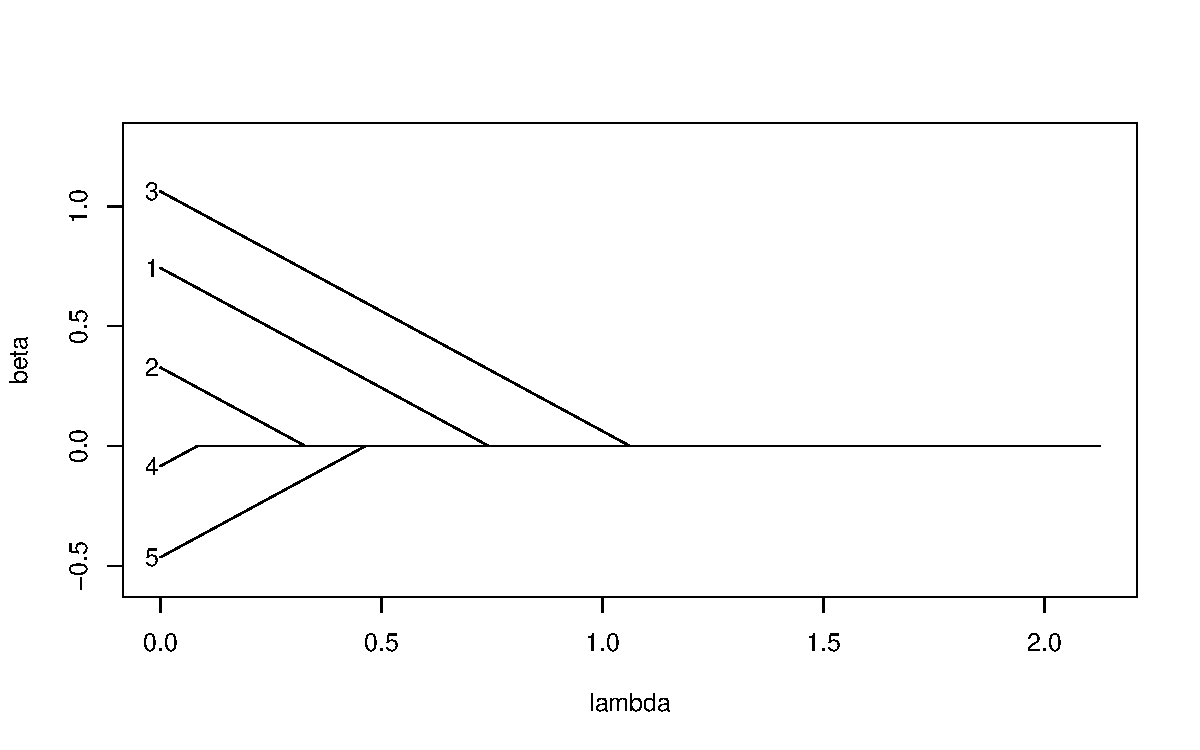
\includegraphics[width=\textwidth]{img/fig04.pdf}
\end{center}

\end{frame}

%%%%%%%%%%%%%%%%%%%%%%%%%%%%%%%%%%%%%%%%%%%%%%%%%%%
\begin{frame}[fragile] \frametitle{}

Recall that only elements $1$ and $3$ of the original
problem were actually non-zero. Look what happens if
we set $\lambda$ to $0.5$.

\end{frame}

%%%%%%%%%%%%%%%%%%%%%%%%%%%%%%%%%%%%%%%%%%%%%%%%%%%
\begin{frame}[fragile] \frametitle{}

\begin{center}
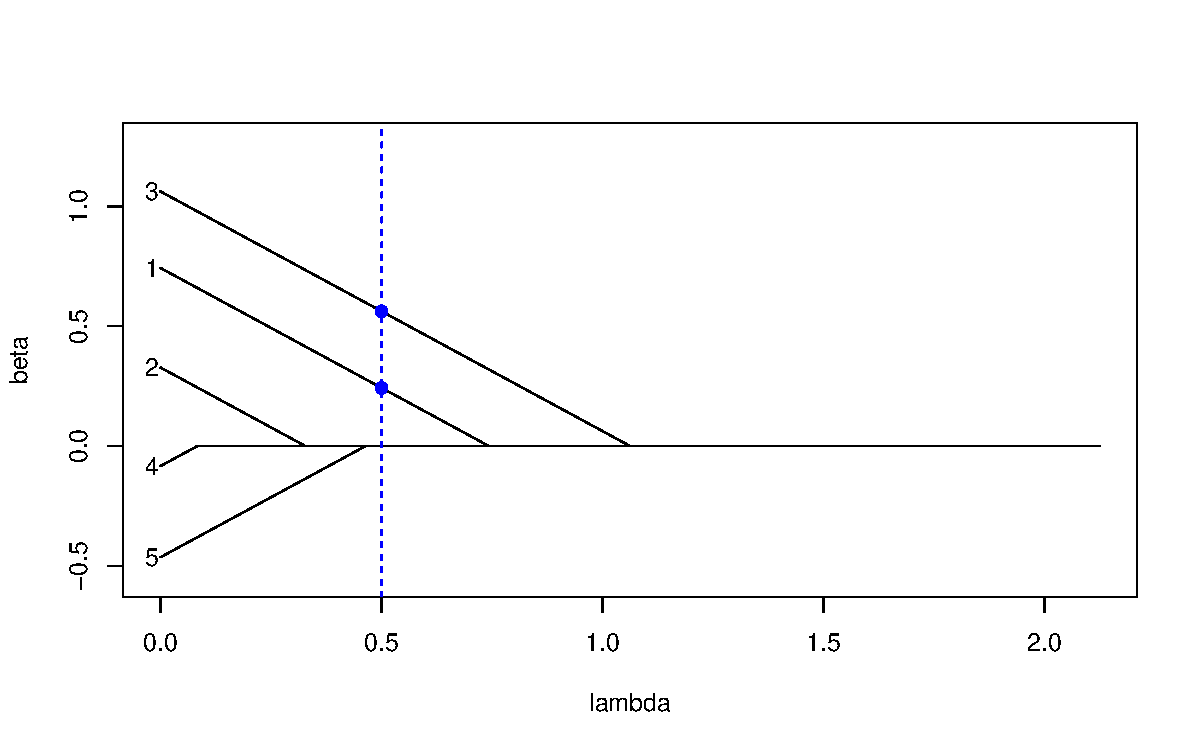
\includegraphics[width=\textwidth]{img/fig05.pdf}
\end{center}

\end{frame}

%%%%%%%%%%%%%%%%%%%%%%%%%%%%%%%%%%%%%%%%%%%%%%%%%%%
\begin{frame}[fragile] \frametitle{}

The \texttt{lars} package, written by the authors of
the aforementioned paper, provides a method for calculating
this without having to write the code manually (and obviously
also handles cases with arbitrary $X^tX$).
\begin{verbatim}
> library(lars)
> out <- lars(X,y,normalize=FALSE,intercept=FALSE)
> out

Call:
lars(x = X, y = y, normalize = FALSE, intercept = FALSE)
R-squared: 0.021
Sequence of LASSO moves:
     3 1 5 2 4
Var  3 1 5 2 4
Step 1 2 3 4 5

> plot(out)
\end{verbatim}


\end{frame}

%%%%%%%%%%%%%%%%%%%%%%%%%%%%%%%%%%%%%%%%%%%%%%%%%%%
\begin{frame}[fragile] \frametitle{}

\begin{center}
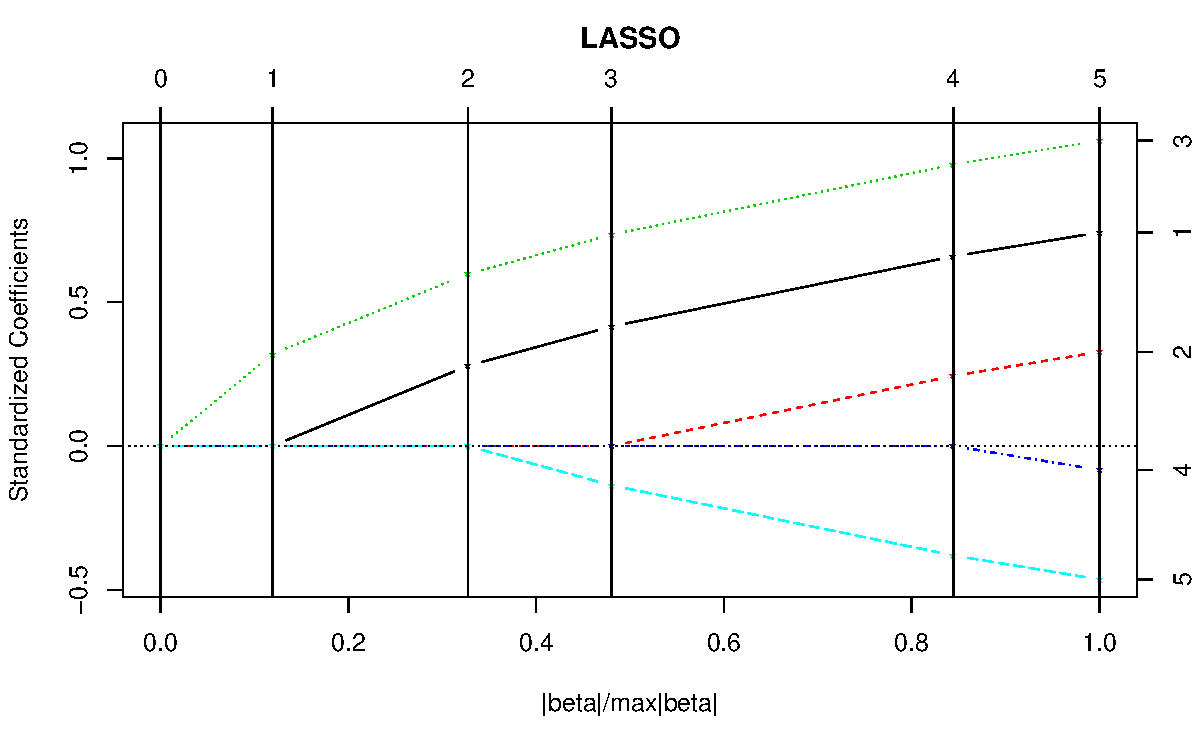
\includegraphics[width=\textwidth]{img/fig06.pdf}
\end{center}

\end{frame}

%%%%%%%%%%%%%%%%%%%%%%%%%%%%%%%%%%%%%%%%%%%%%%%%%%%
\begin{frame}[fragile] \frametitle{}

Turning on the trace feature of lars shows the
path like logic of the algorithm:
\begin{verbatim}
> out <- lars(X,y,normalize=FALSE,intercept=FALSE,
+             trace=TRUE)
LASSO sequence
Computing X'X .....
LARS Step 1 :  Variable 3   added
LARS Step 2 :  Variable 1   added
LARS Step 3 :  Variable 5   added
LARS Step 4 :  Variable 2   added
LARS Step 5 :  Variable 4   added
Computing residuals, RSS etc .....
\end{verbatim}

\end{frame}


%%%%%%%%%%%%%%%%%%%%%%%%%%%%%%%%%%%%%%%%%%%%%%%%%%%
\begin{frame}[fragile] \frametitle{}

What is so much more difficult about the general case?
Consider the function to be minimized:
\begin{align*}
f(b) &= || y - Xb ||_2^2 + 2 \lambda ||b||_1 \\
&= y^t y + b^t X^t X b - 2 y^t X b + 2 \lambda || b ||_1
\end{align*}


\end{frame}

%%%%%%%%%%%%%%%%%%%%%%%%%%%%%%%%%%%%%%%%%%%%%%%%%%%
\begin{frame}[fragile] \frametitle{}

The subdifferential is still fairly easy to calculate,
with the $j$-th component equal to:
\begin{align*}
\partial(h)(b) &= \left\{ \begin{array}{ll}
\left(2 X^t X b - 2 X^t y\right)_{j} + 2\cdot \text{sign}(b_j)\cdot\lambda, & b_j \neq 0 \\[0pt]
\left(2 X^t X b - 2 X^t y\right)_{j} + 2\cdot [-\lambda,\lambda], &b_j = 0
\end{array} \right.
\end{align*}
\pause But consider how hard this is to solve directly now that the
$p$ equations are no longer decoupled given that (1) we need to consider
all permutations of the whether $b_j$ is zero and (2) we have a system
of, possibly, multivalued equations.

\pause The good news is that once we find some $\widehat{\beta}_\lambda$ such
that $\partial(h)(\widehat{\beta}_\lambda)$ contains the zero vector we are
done. No need to calculate or prove anything; a global minimum is assured.

\end{frame}


%%%%%%%%%%%%%%%%%%%%%%%%%%%%%%%%%%%%%%%%%%%%%%%%%%%
\begin{frame}[fragile] \frametitle{}

For example, consider any $\lambda$ greater than $|X^t y|_\infty$ (the
maximum absolute value). I know that $\widehat{\beta}_\lambda$ will be
equal to all zeros, and can show this very quickly as the subdifferential
becomes:
\begin{align*}
\partial(h)(b) &= 2 x_j^t y + 2\cdot[-\lambda,\lambda], &b_j = 0
\end{align*}
\pause Which contains zero because:
\begin{align*}
-\lambda < x_j^t y
\end{align*}
and
\begin{align*}
\lambda > -x_j^t y.
\end{align*}

\end{frame}


%%%%%%%%%%%%%%%%%%%%%%%%%%%%%%%%%%%%%%%%%%%%%%%%%%%
\begin{frame}[fragile] \frametitle{}

Now, assume that the values of $X^t y$ are unique, positive,
and ordered from highest to lower values. These conditions
simply keep the notation easier, with all but the uniqueness
being easy to account for with a few more conditional statements.

\end{frame}


%%%%%%%%%%%%%%%%%%%%%%%%%%%%%%%%%%%%%%%%%%%%%%%%%%%
\begin{frame}[fragile] \frametitle{}

It turns out that for $\lambda$ between $x_1^t y$ and
$x_2^t y$, we get the same solution as in the uncorrelated
case (with the addition of scaling factor as $x_1^t x_1$ may
not be $1$):
\begin{align*}
\widehat{\beta}_\lambda &= \frac{1}{x^t_1 x_1} \cdot \left(\begin{array}{c}
x_1^t y - \lambda \\
0\\
\vdots\\
0
\end{array} \right)
\end{align*}
This can be shown fairly easily by plugging into the subdifferential
equation.

\end{frame}

%%%%%%%%%%%%%%%%%%%%%%%%%%%%%%%%%%%%%%%%%%%%%%%%%%%
\begin{frame}[fragile] \frametitle{}

For $j$ not equal to $1$, we will have:
\begin{align*}
0 \in 2 x_j^t y + 2\cdot[-\lambda,\lambda]
\end{align*}
Because $\lambda > x_j^t y$, as the inner products are sorted from
largest to smallest.

\end{frame}

%%%%%%%%%%%%%%%%%%%%%%%%%%%%%%%%%%%%%%%%%%%%%%%%%%%
\begin{frame}[fragile] \frametitle{}

For the $j=1$ case, we have:
\begin{align*}
0 &= \left(2 X^t X b - 2 X^t y\right)_{j} + 2\cdot \text{sign}(b_j)\cdot\lambda \\
0 &= 2 x^t_1 x_1 b_1 - 2 x_1^t y + \lambda \\
b_1 &= \frac{1}{x^t_1 x_1} \left( x_1^t y - \lambda \right)
\end{align*}
Which finishes the result.

\end{frame}


%%%%%%%%%%%%%%%%%%%%%%%%%%%%%%%%%%%%%%%%%%%%%%%%%%%
\begin{frame}[fragile] \frametitle{}

For values with $x_3^t y \leq \lambda \leq x_2^t y$, the solution
for $\widehat{\beta}$ linear with non-zero elements in just the
first $2$ components.

\pause The details from there on out are what is covered on problem
set $6$.

\end{frame}

%%%%%%%%%%%%%%%%%%%%%%%%%%%%%%%%%%%%%%%%%%%%%%%%%%%
\begin{frame}[fragile] \frametitle{}

As a final example, we'll construct some correlated data with a
sparse model and show what the lars path solution looks like:
\begin{verbatim}
> n <- 1000
> p <- 25
> X <- matrix(rnorm(p*n),ncol=p)
> X <- X*0.8 + X[,1]*0.2
> beta <- sample(0:1,p,replace=TRUE,prob=c(9,1))
> which(beta != 0)
[1] 14 20
> y <- X %*% beta + rnorm(n,sd=0.3)
\end{verbatim}

\end{frame}

%%%%%%%%%%%%%%%%%%%%%%%%%%%%%%%%%%%%%%%%%%%%%%%%%%%
\begin{frame}[fragile] \frametitle{}

\begin{center}
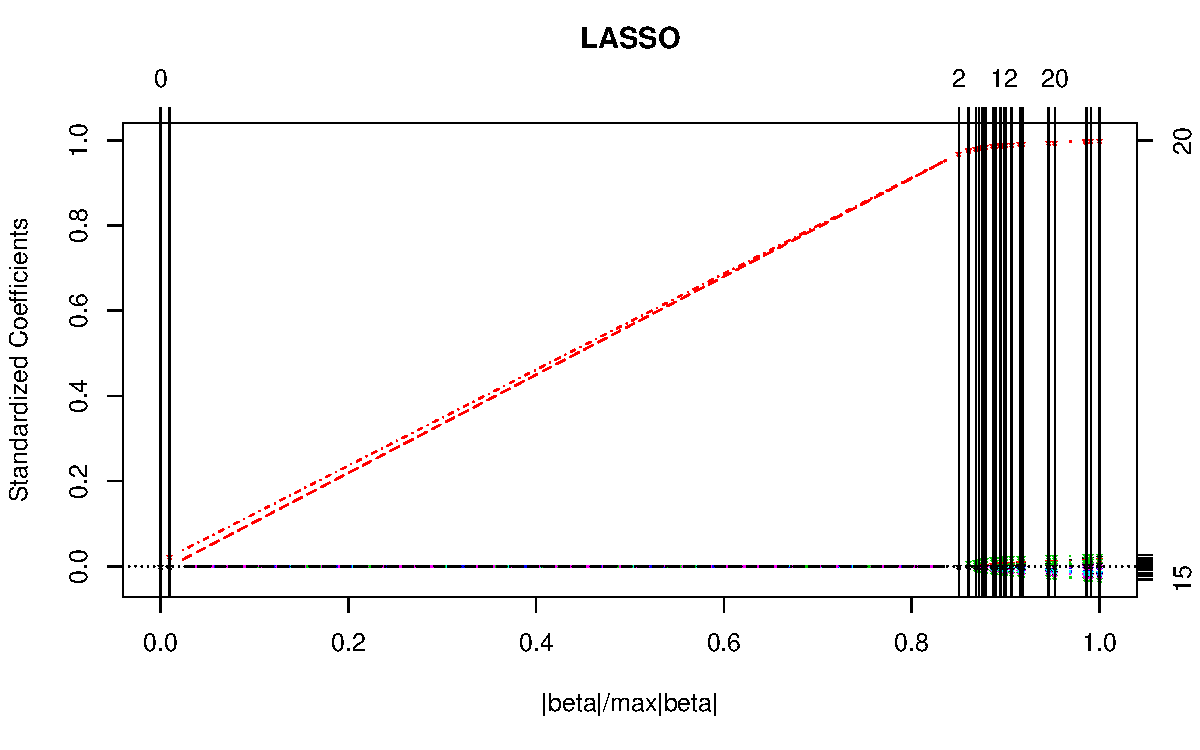
\includegraphics[width=\textwidth]{img/fig07.pdf}
\end{center}

\end{frame}

\end{document}











